\documentclass[a4paper,11pt, twocolumn]{article}
\usepackage[margin=0.8in]{geometry}
\usepackage{xcolor}
\usepackage{graphicx} %package to manage images
\graphicspath{ {./images/} }
\usepackage{float}

\title{1.2.3 Software Development}
\author{Revision sheet}
\date{}

\usepackage{fancyhdr}
\pagestyle{fancy}
\fancyhead{} % clear all header fields
\renewcommand{\headrulewidth}{0pt} % no line in header area
\fancyfoot{} % clear all footer fields
\renewcommand{\footrulewidth}{0.4pt}
\fancyfoot[C]{\thepage} % page number in centre of the page
\fancyfoot[R]{\footnotesize Thomas Boxall \\ Images from the textbook} % right hand footer has author name on top line and images reference on bottom line
\fancyfoot[L]{\footnotesize 1.2.3 Software Development \\ Revision sheet} % left hand footer has title of document on top line and 'Revision Sheet' on bottom line


\begin{document}

\maketitle
\thispagestyle{fancy}

% CONTENTS OF THE REVISION SHEET HERE

\section{Systems Analysis}
Software development is the process which is gone through to develop any piece of software. There are a number of different methodologies which can be used, each of them have common stages.
\subsection{Analysis}
Before the problem can be solved, it has to be defined. The requirements of the system that solves the problem must be established, this could include: data (what will it be, where it comes from, how much there is); procedures (what is done, where, when and how is it done, how errors and exceptions are handled); future (development plans and expected growth rates); and problems (with existing solutions). Many similar problems (for example, games) will have a similar set of requirements.
\subsection{Design}
Depending on the type of the project, some or all of the following may need to be designed: processing (what o the algorithms do); data structures (how will the data be stored); output (how the program will output); input (how will this be handled); user interface (what the system will look like to users, how they will interact with it); security (how is the data going to be kept secure); and hardware (selection of the appropriate configuration).
\subsection{Programming}
Now the system has been designed, it can be programmed. This usually involves breaking down the problem into individual modules which each perform a single well-defined task. The following stage, testing is closely intertwined with programming.
\subsection{Testing}
Before a system can be put into production use, it has to be tested to make sure that all errors are discovered and fixed. As part of the design, a test plan should be written which ensures all parts of the system are thoroughly tested. The plan may make use of all or some of the following.
\subsubsection{Black Box Testing}
Also known as functional testing. This is where someone independent of the implementation team runs through a test plan containing inputs and outputs, recording them. The tests focus on the function of the program - is it producing the right output for the input.
\subsubsection{White Box Testing}
Also known as structural testing. This testing is dependent on the code logic and is derived from the program structure rather than the function. The program code is studied and each path through it is tested. A disadvantage to this is that you can't test what isn't there.
\subsubsection{Alpha Testing}
This is carried out by the software developers in-house testing team. It often reveals errors and omissions in the systems requirements. The user may find that the program doesn't have the required functionality because the requirements were not specified carefully enough or because the developer has missed or misunderstood something in the specification. 
\subsubsection{Beta Testing}
This is where the new package is given to a number of users who can review the software and report bugs to the developer. It exposes the product to real users and detects problems and errors that my not have been anticipated by the developer. The product can be modified and sent out for further beta testing until the developer is confident enough in the product that it can be put on the market.
\subsection{Implementation}
After all the programming and testing is done, the software can be installed on the user's system and more testing done. It is usual at this stage for different weaknesses and omissions to be found, these will be improved upon.
\subsection{Evaluation}
The evaluation stage can be carried out a few months after implementation. This gives people using the system a chance to understand how it works and get used to using it. This will also give the users a chance to identify any shortcomings of the system. The system should be evaluated on the basis of effectiveness, usability and maintainability. The post-implementation review will focus on: comparing the systems actual performance to its designed performance; errors which were introduced during system development; unexpected benefits and problems.

\section{System Development Lifecycles}
\subsection{Waterfall Model}
In this methodology, each step is completed fully before moving onto the next. Each step has specific outputs that lead into the next step, due to this, if you need to return to a previously completed step then you have to go back down through all of the following steps again. The clients are involved at the beginning of the process (in the analysis stage) but then have no involvement until the evaluation stage. It is still popular now however, more effective models are used more commonly.
\begin{figure}[H]
    \centering
    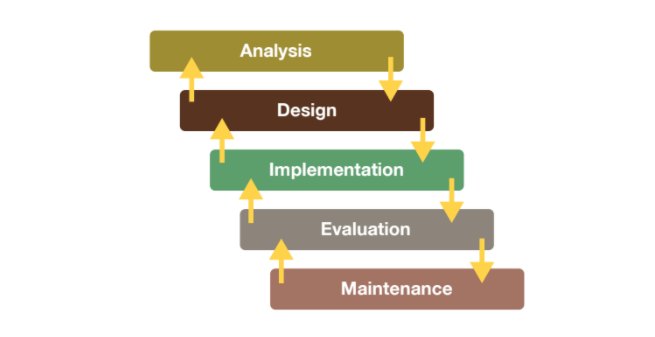
\includegraphics[width=0.45\textwidth]{images/waterfall.png}
    \caption{Waterfall lifecycle}
    \label{fig:waterfall}
\end{figure}
\subsection{Spiral Model}
This uses the same structured steps but repeats them, developing the software iteratively. Each loop around the spiral develops the prototype more until the product is finished. The spiral model also has a large focus on risk, analysing and managing it at every stage. This is commonly used for large projects which may take years to deliver. 
\begin{figure}[H]
    \centering
    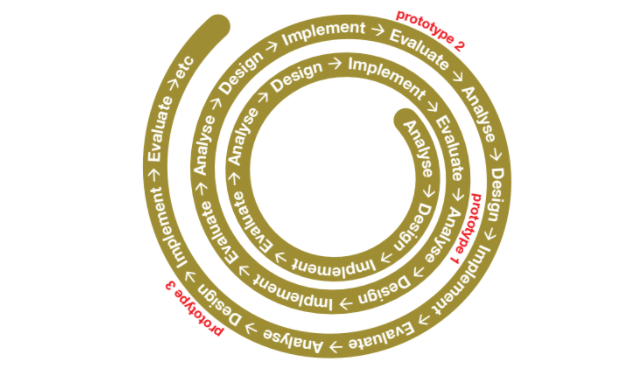
\includegraphics[width=0.45\textwidth]{images/spiral.png}
    \caption{Spiral lifecycle}
    \label{fig:spiral}
\end{figure}
\noindent Each time around the spiral, the following happens: analyse requirements for next prototype; design the new prototype; implement the new prototype; evaluate the new prototype. 
\subsection{Agile Model}
In this model, all the stages are not completed in sequence. This methodology allows some analysis to be done, then that to be designed and implemented. Feedback from the user is fundamental to this methodology, with the user involved throughout the process. At the start of the process, it is usual for the developers to do just enough modelling so that the requirements are understood by themselves and by the client.
\begin{figure}[H]
    \centering
    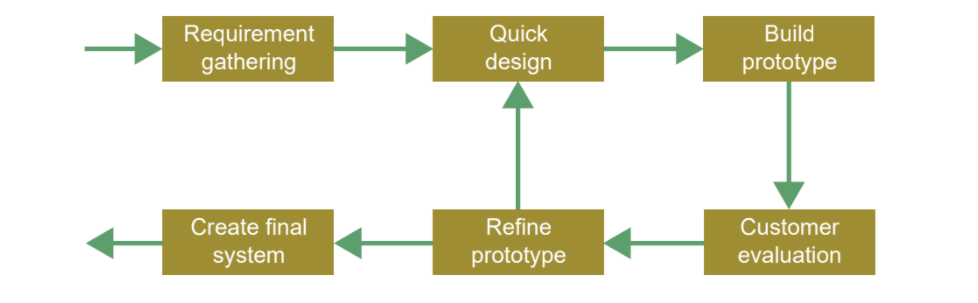
\includegraphics[width=0.45\textwidth]{images/agile.png}
    \caption{Agile lifecycle}
    \label{fig:agile}
\end{figure}
\noindent At each stage of the process, a prototype is built. This ensures that the software is inline with what the user wants. The success of the model depends on: keeping the model simple, rapid feedback from the user, understanding that the users requirements may change and being prepared to make incremental changes as the model develops.
\subsection{Extreme Programming}
This intends to improve software quality and responsiveness to changes in the customers requirements. It is based off of agile software development in `releases' of the software are made in short development cycles. This improves productivity and introduces checkpoints at which new customer requirements can be adopted. This may involve pair programming, which is where two people use one computer - where one is typing and the other is watching. This reduces the chances of bugs and increases the chance of a better algorithm being written.
\subsection{Rapid Application Development}
This was introduced to resolve problems which occurred with projects where systems were being developed over a number of years, during which time requirements and technology changed. The RAD methodology focuses on rapid completion of major projects, using the following principles: workshops and small group conversations to gather requirements rather than formal documentation; continuous prototyping so that users are involved at every stage; producing each part of the system within a strict time limit - some elements of the system may not be perfect but they will be `good enough'; and to reuse software components which have been used elsewhere.
\subsection{Comparison Of The Methodologies}
Waterfall is suitable for very small projects which require supervision. For example, a project undertaken by students or trainees. The major drawback is that the user is not involved much.\newline
Spiral and Agile improve on Waterfall as they acknowledge the users lack of computational thinking, then allow them to be involved during the development process more - building useful prototypes which users can comment on rather than allowing them to just state a requirement at the start.\newline
Extreme programming and RAD are good for large projects where there is a danger of being bogged down or sidetracked. 

\section{Installation Methods}
There are a number of different methods which can be used for the installation/ deployment of software.
\subsubsection*{Phased}
Small parts of the system are introduced to the whole user base over time. This helps to pinpoint errors.
\subsubsection*{Pilot}
The entire system is introduced to one part of the business. This will only introduce errors to one part of the business (if there are any). Pilot deployment is usually done as part of User Acceptance Testing. If the system is deemed not fit for purpose, it is easy to roll-back to the old system as only one part of the business is using the new system.
\subsubsection*{Direct}
The entire business moves instantly over to the new system.

\section{Maintenance Of Systems}
After deployment, a system will need to be maintained. There are three types of updates which can be deployed.
\subsubsection*{Adaptive}
Updating the system for a future need. For example, adding a new map to a video game.
\subsubsection*{Reflective}
Updating the system to make it better. For example, simplify the algorithms to get a better Big O value.
\subsubsection*{Corrective}
Its broken and needs fixing.

\end{document}

(a) Understand the waterfall lifecycle, agile
methodologies, extreme programming, the spiral
model and rapid application development.
(b) The relative merits and drawbacks of different
methodologies and when they might be used.
(c) Writing and following algorithms.